\documentclass[12pt]{article}
% Set font to Times (similar to Times New Roman)
\usepackage[T1]{fontenc}
\usepackage{mathptmx}
% Set font size sections and subsections
\usepackage{sectsty}
\sectionfont{\fontsize{16}{15}\selectfont}
\subsectionfont{\fontsize{16}{15}\selectfont}
% Set document margins to 3cm
\usepackage[margin=3cm]{geometry}
\usepackage{cite}
\usepackage{amsmath,amssymb}
\usepackage{ctable}
\usepackage{tabularx}
\usepackage{float}
\usepackage[sc]{caption}
\usepackage{multirow}
\usepackage{microtype}
\usepackage{epstopdf}
\usepackage{verbatim}
\usepackage{verbatimbox}
\usepackage[multiple,bottom]{footmisc}
\usepackage[title,titletoc,toc]{appendix}
\usepackage{setspace}
\usepackage{rotating}
\usepackage{lscape}
%\usepackage{pdflscape}
\usepackage{subfigure}
\usepackage[para,online,flushleft]{threeparttable}
\usepackage{hyperref}
\usepackage{bm}
\usepackage{ragged2e}
\usepackage{epsf} 
\usepackage{graphicx}
\setlength{\parskip}{1em}
\setlength{\parindent}{0em}

\usepackage{bbold}
\usepackage[utf8]{inputenc}
\usepackage[english]{babel}
\setcounter{MaxMatrixCols}{20}
% Set footnote indent preferences
\makeatletter
\renewcommand\@makefntext[1]{\leftskip=0.5em\hskip0em\@makefnmark#1}
\makeatother
\addtolength{\footnotesep}{2mm}
% Set hyperlink looks
\hypersetup{colorlinks,urlcolor=blue,citecolor=black,linkcolor=black}
\makeatletter
\renewcommand*{\@cite@ofmt}{\bfseries\hbox}
\makeatother
\urlstyle{same}
%Para settings
\setlength\parindent{0pt}
\linespread{1.1}
% Biblio settings
\usepackage{natbib}
% Captions & Sources style
\usepackage[margin={2cm,2cm},labelfont=bf, font=small,justification=raggedright,singlelinecheck=false]{caption}
\newcommand{\source}[1]{\vspace{-3pt} \caption*{ Source: {#1}} }
% Set footnote size
\renewcommand{\footnotesize}{\small}

% Title, author, date
\author{Author: Ivan Vallejo Vall \\ Tutor: Iñigo Herguera García}
\title{%
  \vspace{-0.0cm}MASTER PROJECT \\ 
  \vspace{1cm} Measuring real broadband speeds using \\ crowdsourcing data from the Internet Foundation \\ \vspace{2cm} 
  }
\date{\vspace{1cm} Data Science Program 2016/2017 \\ 
\vspace{2cm} 
\includegraphics[scale=0.5]{Logo_GSE_green.png}}


\begin{document}
\linespread{1.4}\selectfont
\pagenumbering{gobble}% Remove page numbers (and reset to 1)
\maketitle
\newpage
\begin{abstract}
   Here goes the abstract-text, max 150 words.
\end{abstract}
\newpage
\tableofcontents
\newpage
\listoffigures
\newpage
\pagenumbering{arabic}% Arabic page numbers (and reset to 1)
\section{Introduction}
\subsection{Background}
The International Telecommunication Union -- ITU, the United Nations specialized agency for information and communication technologies (ICTs)\footnote{For more information on ITU, see \href{http://www.itu.int/en/about/Pages/default.aspx}{ITU's website}} -- is carrying out a series of pilot studies under the umbrella of the project Big Data for Measuring the Information Society (\autoref{fig:a1}).\footnote{For more information on the ITU project Big Data for Measuring the Information Society, see its \href{http://www.itu.int/en/ITU-D/Statistics/Pages/bigdata/default.aspx}{website}.} 
\vspace{1cm}
\begin{figure}[H]
    \centering
        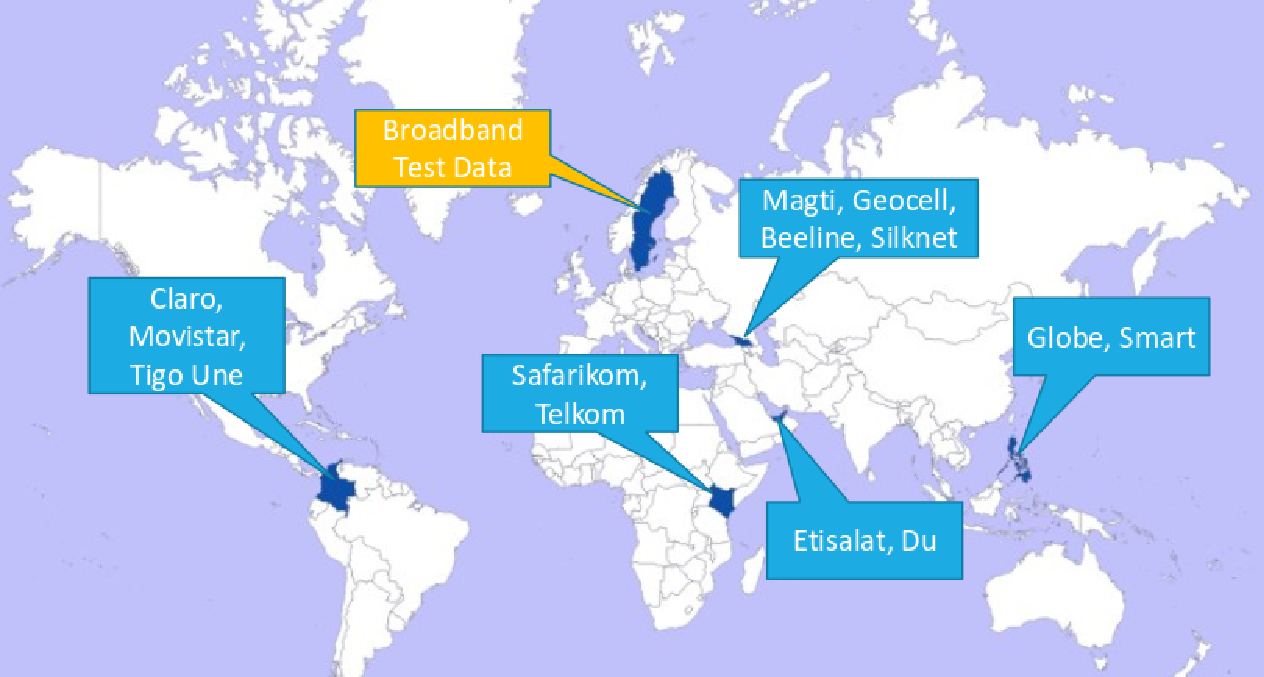
\includegraphics[width=\linewidth]{itu_projects.pdf}
        \caption{Big Data for Measuring the Information Society -- ITU pilot projects.}
        \caption*{\textbf{Source:} \cite{margus}.}
        \label{fig:a1}
\end{figure}   


The objective of the project is to show how big data from the telecommunication industry can be used to produce new ICT indicators and replace or complement existing ones with a view to measuring the development of the Information Society worldwide. 

In particular, these pilot studies aim to be a first step towards filling in the ICT data gaps in the global indicator framework agreed for the monitoring of the 2030 Agenda for Sustainable Development \citep{interagency}, and to inform private and public stakeholders on the current status of the digital divide.      

The object of this master thesis concerns the measurements on broadband speeds carried out by the Internet Foundation in Sweden (IIS) and made available to ITU in the context of the project Big Data for Measuring the Information Society.    

\subsection{Relevance}
Broadband speed measurements matter because they are a key input for several consumer, policy and regulatory decisions:

\begin{itemize}

	\item From a \textbf{consumer perspective}, broadband speed is one of the most important factors when choosing an Internet connection. For instance, in the European Union (EU) the download speed is the second most cited factor, after price, when deciding which broadband plan to choose.\footnote{On average, 41 per cent of respondents in the EU mentioned download speed as an important factor factor when subscribing to an Internet connection, compared with 71 per cent of respondents citing price. The figures refer to fieldwork carried out in January 2014.} However, six out of ten EU citizens do not know the maximum download speed of their broadband Internet plan and, among those that know it, a quarter of them believe that their real speed does not correspond to the one specified in their contract. Moreover, four in ten households in the EU admit having experienced difficulties accessing content at home because of speed or capacity issues \citep{eurobarometer}. It can thus be concluded that Internet speed is an important and controversial factor for consumers. 
	
	\item From a \textbf{regulatory perspective}, broadband speed is one of the parameters often monitored to ensure that telecommunication operators and Internet service providers (ISPs) comply with some minimum quality-of-service (QoS) requirements. For example, Spain regulates the QoS parameters of electronic communication services by means of a service order, which includes specific Internet access parameters \citep[Annex I, Part II in ][]{boe}. In a similar fashion, the Telecom Regulatory Authority of India sets that subscribers should get a minimum of 80 per cent of the speed in their contract, as measured from the ISP node to the user \citep{trai2006}.         
	
	\item From a \textbf{policy perspective}, broadband speeds have wide implications concerning the initiatives undertaken in the telecommunication sector. For instance, the definition of broadband is often tied to a given minimum speed, which is subject to be revised, as was the case in India in 2014 (from 256 to 512 kbit/s) \citep{trai2014}. In the United States, the Congress asked the Federal Communications Commission (FCC) to evaluate the deployment of \textit{advanced telecommunication capabilities}. FCC considered these capabilities to require 4 Mbit/s download and 1 Mbit/s upload speeds in 2010, but revised the benchmark speeds to 25 Mbit/s download and 3 Mbit/s upload in 2015 \citep{fcc2015a}. In Europe, Finland was a worldwide pioneer in declaring affordable broadband access a basic right in 2010. Finland's Ministry of Transport and Communications set the threshold for the basic connection to 1 Mbit/s in 2010, revising it to 2 Mbit/s in 2016 \citep{eprs}. All these policy decisions have deep economic implications. Indeed, in most cases they imply the mobilization of universal service funds (USF) or subsidy schemes to meet the targets set in terms of availability of affordable Internet connections at a given speed.        
\end{itemize}

In addition to these consumer, policy and regulatory implications, broadband speeds may also be an important determinant of broadband impact on economic growth \citep{bohlin2012}. Higher broadband speeds have also been found to be causally linked to increases in the percentage of employees classified as creative class workers \citep{whitacre2014}. 

All these factors motivate the interest in producing accurate data on actual broadband speeds.     

\subsection{Research questions}
\vspace{1cm}
\setlength{\fboxsep}{1em}
\centerline{\fbox{\begin{minipage}{0.8\linewidth}
\begin{enumerate}
\item Can crowdsourcing Internet data be used to measure real broadband speeds?
\item Which information can be extracted from online speed measurements to characterize Internet users?   
\end{enumerate}
\end{minipage}}}
\vspace{1cm}
Given the relevance of broadband speeds for consumers, regulators and policy-makers, there is a growing demand for accurate measurements. 

Advertised speeds, as publicized by operators and ISPs, provided only an upper-limit to the actual broadband speeds. On the other hand, precise external hardware-based measurements, such as the ones commissioned to SamKnows by the regulatory agencies in the UK \citep{ofcom2017}, the United States \citep{fcc2015b} and the European Commission \citep{samknows2013} are costly. Therefore, they cannot be realistically scaled up to a wider set of countries.  

Software-based, crowdsourcing data on Internet speed measurements remains the only possible stable source of real broadband speed information for most countries. Moreover, the low cost of deployment of these measurement platforms makes it possible to envisage its adoption by any interested regulator/policy-making. 

Indeed, some regulators in developing countries, such as the Telecommunications Regulatory Commission of Sri Lanka, have already launched their own measurement portal (\autoref{fig:a2}). Moreover, there are private stakeholders, such as Ookla, recording these data at the global level.\footnote{For more information on Ookla's Speedtest, see \autoref{meth} and \href{http://beta.speedtest.net/about}{Speedtest website}.} 

\begin{figure}[H]
    \centering
        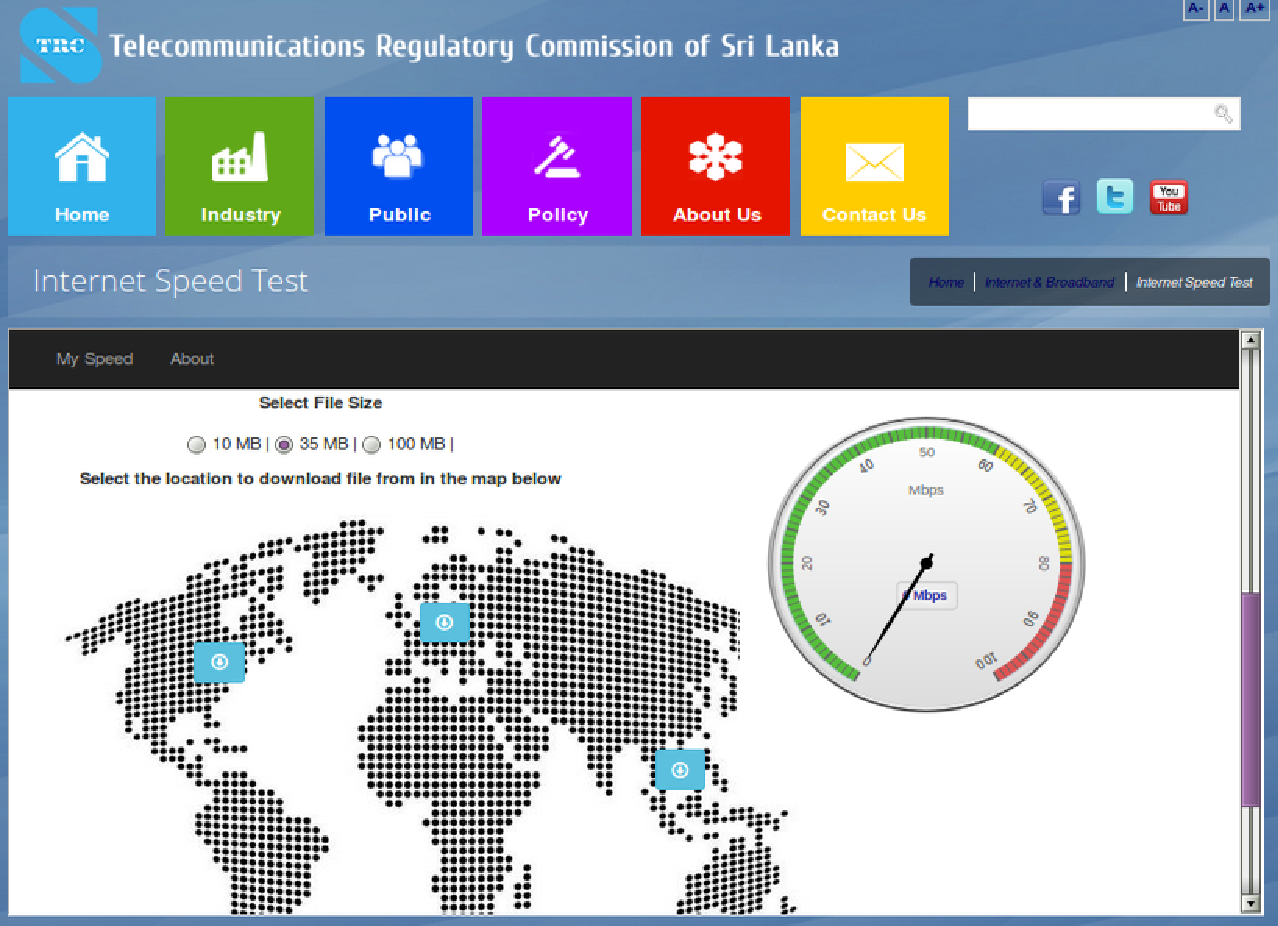
\includegraphics[width=\linewidth]{srilanka.pdf}
        \caption{Internet Speed Test Platform,  Sri Lanka.}
        \caption*{\textbf{Source:} \href{http://www.trc.gov.lk/2014-05-12-13-25-54/internet-speed-test.html}{Telecommunications Regulatory Commission of Sri Lanka}.}
        \label{fig:a2}
\end{figure}   

\textbf{Because of this... bla bla}

\section{State of the art}
Start by mentioning advertized speeds...
\subsection{Measurement methodologies} \label{meth}
Bla bla
\subsection{Statistical approach}
Bla bla
\section{Data}
Bla bla
\subsection{Processing environment}
Bla bla
\section{Results}
Bla bla
\section{Conclusion}
Bla bla

\nocite{*}

\bibliography{references}
\bibliographystyle{apalike}


\end{document}